%%%%%%%%%%%%%%%%%%%%%%%%%%%%%%%%%%%%%%%%%%%%%%%%%%%%%%%%%%%%
%%  This Beamer template was created by Cameron Bracken.
%%  Anyone can freely use or modify it for any purpose
%%  without attribution.
%%
%%  Last Modified: January 9, 2009
%%

\documentclass[xcolor=x11names,compress]{beamer}

%% General document %%%%%%%%%%%%%%%%%%%%%%%%%%%%%%%%%%
\usepackage{graphicx}
\usepackage{tikz}
\usepackage{fontawesome}
\usepackage{siunitx}
\usepackage{outlines}
\usepackage{enumitem}
\usepackage{pgfplots}
\usepackage{subfig}
\usetikzlibrary{decorations.fractals}
%%%%%%%%%%%%%%%%%%%%%%%%%%%%%%%%%%%%%%%%%%%%%%%%%%%%%%


%% Beamer Layout %%%%%%%%%%%%%%%%%%%%%%%%%%%%%%%%%%
\useoutertheme[subsection=false,shadow]{miniframes}
\useinnertheme{default}
\usefonttheme{serif}
\usepackage{palatino}

\setbeamerfont{title like}{shape=\scshape}
\setbeamerfont{frametitle}{shape=\scshape}

\setbeamercolor*{lower separation line head}{bg=DeepSkyBlue4} 
\setbeamercolor*{normal text}{fg=black,bg=white} 
\setbeamercolor*{alerted text}{fg=red} 
\setbeamercolor*{example text}{fg=black} 
\setbeamercolor*{structure}{fg=black} 

\setbeamercolor*{palette tertiary}{fg=black,bg=black!10} 
\setbeamercolor*{palette quaternary}{fg=black,bg=black!10} 

%%%%%%%%%%%%%%%%%%%%%%%%%%%%%%%%%%%%%%%%%%%%%%%%%%
\author{Lorenz Schmidt \inst{1} \and Paul Koerbitz \inst{2}}
\institute{\it \inst{1} RWTH Aachen \and \inst{2} Google}

\setlist[itemize]{label=$\blacktriangleright$}
\begin{document}

%%%%%%%%%%%%%%%%%%%%%%%%%%%%%%%%%%%%%%%%%%%%%%%%%%%%%%
%%%%%%%%%%%%%%%%%%%%%%%%%%%%%%%%%%%%%%%%%%%%%%%%%%%%%%
\section{Outline}
\begin{frame}
    \title{Linfa}
    \subtitle{Classical Machine Learning with Rust}
    \date{
        
\includegraphics[scale=0.5]{images/rust.png} \\
        \vspace{0.5cm}
        \today
    }
	\titlepage
\end{frame}

%%%%%%%%%%%%%%%%%%%%%%%%%%%%%%%%%%%%%%%%%%%%%%%%%%%%%%
%%%%%%%%%%%%%%%%%%%%%%%%%%%%%%%%%%%%%%%%%%%%%%%%%%%%%%f
\begin{frame}{Introduction}
	\tableofcontents
\end{frame}

\begin{frame}{classical machine learning}
    \frametitle{Classical Machine Learning}

    \begin{itemize}
        \item<1-> Don't the cool kids use neural nets these days?
    \only<2>{
        \begin{figure}[ht]
            \centering
            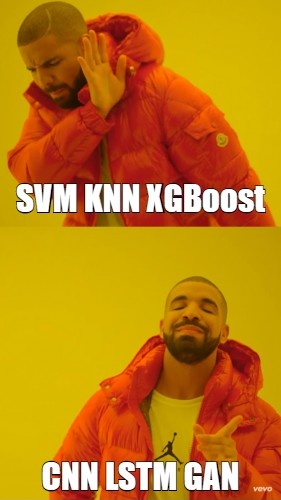
\includegraphics[width=0.3\linewidth]{images/meme1.png}
        \end{figure}
    }
        \item<3-> \textit{PCA}, \textit{SVM}, \textit{ElasticNet}, \textit{kernel methods}, \dots
        \item<4-> But still easier to interpret and faster if domain suits
    \end{itemize}

\end{frame}

\begin{frame}{aim of linfa}
    \frametitle{Why Linfa?}
    Why do classical ML in Rust? Doesn't scikit-learn solve everything?
    \begin{itemize}
        \item<2-> Rust as a universal implementation language
            \only<3>{
                \begin{figure}[ht]
                    \centering
	            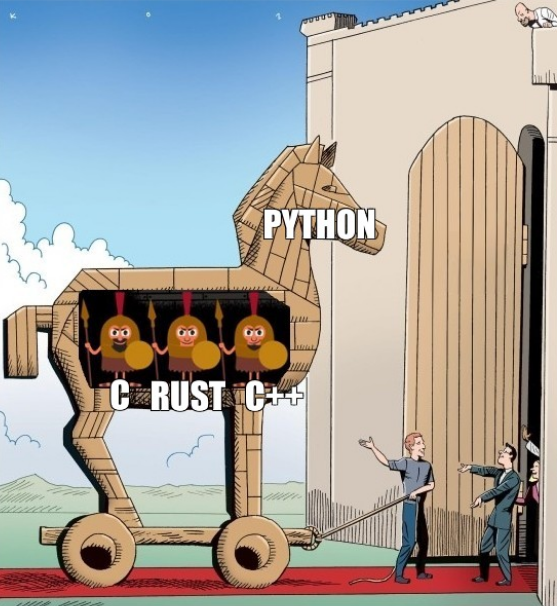
\includegraphics[width=0.45\linewidth]{images/workhorse.png}
                \end{figure}
            }
        \begin{itemize}[label=-]
            \item<4->{Efficient, no GC, no runtime}
	    \item<5->{Use borrowing system helps avoiding accidental copies}
	    \item<5->{Rust has nice things ... compiler, IDE, package mgmt, testing, benchmarking, ...}
	    \item<6->{... much nicer than C, C++, Fortran, ...}
        \end{itemize}
	    \item<7-> Rust for performance critical situations
        \begin{itemize}[label=-]
            \item<8->{Large scale ML applications}
	    \item<9->{Low memory environments (IoT)}
        \end{itemize}	
    \end{itemize}
\end{frame}

\begin{frame}{aim of linfa}
    \frametitle{Why Linfa?}
    Why now? Why this project (Linfa)?
    \begin{itemize}
        \item<2-> Timing: Prerequisites are now met
        \begin{itemize}[label=-]
            \item<3->{Matrix libraries}
	    \item<4->{Optimization libraries}
	    \item<5->{...}
        \end{itemize}
        \item<6->{Linfa is a community effort}
        \begin{itemize}[label=-]
            \item<7->{Started by Luca Palmeri at RustFest 2019 with the explicit goal of being a community effort ...}
	    \item<8->{... now hosted by the Rust ML WG ... }
	    \item<9->{... and developed by a number growing number of contributers.}
        \end{itemize}	
    \end{itemize}
\end{frame}

\section{Interfaces}

\begin{frame}{classes}
    \frametitle{Classes of Algorithms}

    \onslide<2->{
    \begin{minipage}{0.55\linewidth}
        $\blacktriangleright$ Examples
        \only<2>{
        \begin{itemize}[label=-]
            \item Kernel methods
            \item \textit{PCA}, Diffusion maps
            \item t-SNE
        \end{itemize}
        }
        \only<3>{
        \begin{itemize}[label=-]
            \item Decision trees
            \item Hierarchical clustering
            \item DBSCAN, Optics
        \end{itemize}
        }

        \only<4>{
        \begin{itemize}[label=-]
            \item ElasticNet
            \item Gaussian mixture model
            \item Fast ICA
        \end{itemize}
        }
    \end{minipage}
    \begin{minipage}{0.40\linewidth}
        \begin{figure}[ht]
            \centering
            \resizebox{0.75\linewidth}{!}{\begin{tikzpicture}
  \begin{scope}[blend group = soft light]
    \fill[red!30!white]   ( 90:1.2) circle (3);
    \only<3->{\fill[green!30!white] (90:1.2) circle (2);}
    \only<4->{\fill[blue!30!white]  (90:1.2) circle (1.1);}
  \end{scope}
  \node at ( 90:3.6)    {Transformer};
  \only<3->{\node at ( 90:2.6)   {Fittable};}
  \only<4->{\node at ( 90:1.2)   {Incremental};}
\end{tikzpicture}
}
        \end{figure}
    \end{minipage}
    }
    \begin{minipage}[b][4cm][b]{\textwidth}
    \only<2>{
        \begin{figure}[ht]
            \centering
            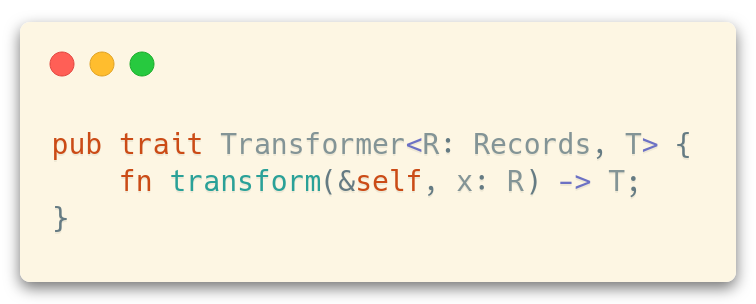
\includegraphics[width=0.5\linewidth]{images/classes1.png}
        \end{figure}
    }
    \only<3>{
        \begin{figure}[ht]
            \centering
            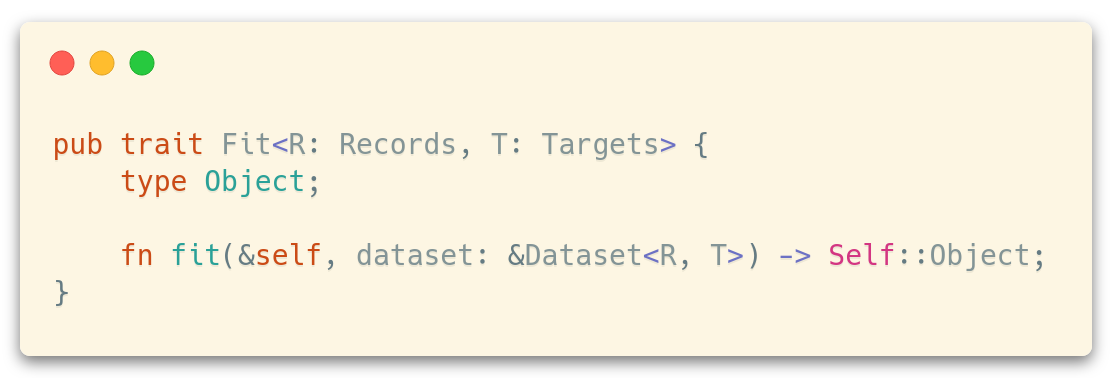
\includegraphics[width=0.7\linewidth]{images/classes2.png}
        \end{figure}
    }
    \only<4>{
        \begin{figure}[ht]
            \centering
            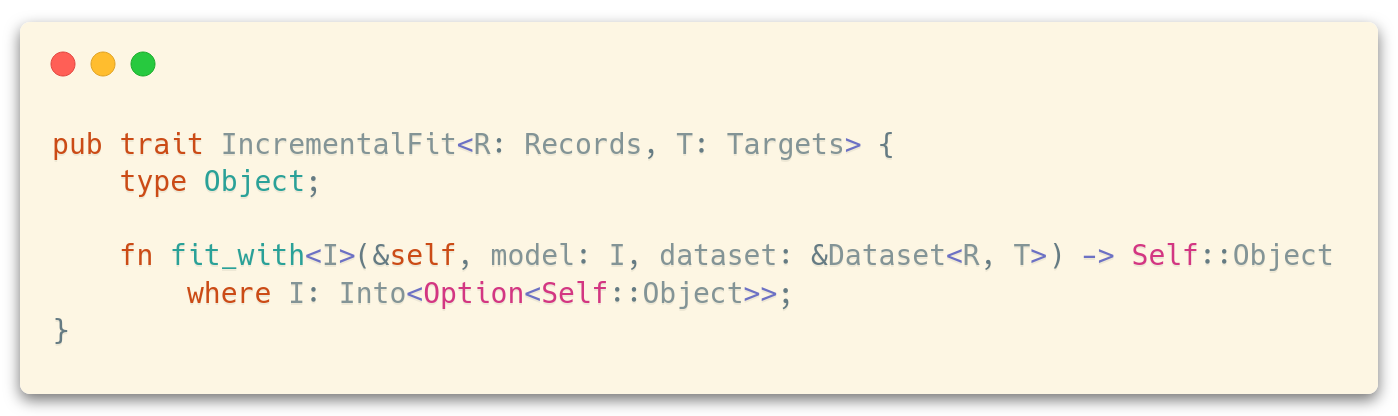
\includegraphics[width=0.85\linewidth]{images/classes3.png}
        \end{figure}
    }
    \hspace{3em}
    \end{minipage}
\end{frame}

\begin{frame}{datasets}
    \frametitle{Dataset}

    \begin{itemize}
        \item<1-> Offer unified interface for data and targets
        \item<2-> Associated types for late binding in \textit{Records}, \textit{Targets} traits
        \only<2>{
            \begin{figure}[ht]
                \centering
                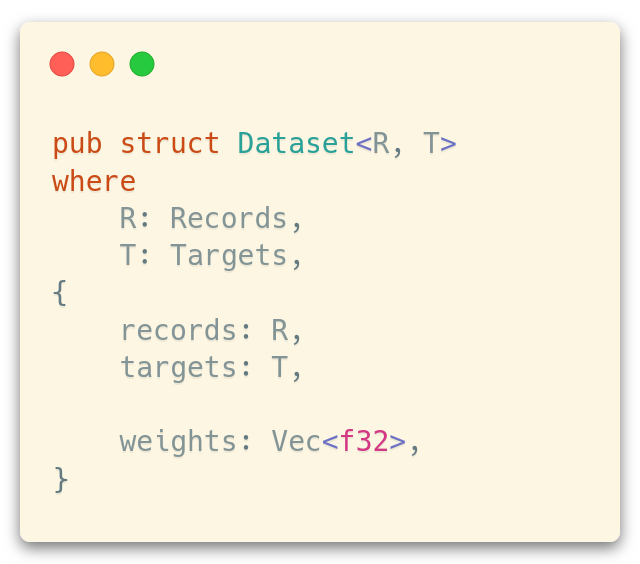
\includegraphics[width=0.5\linewidth]{images/dataset_def.png}
            \end{figure}
        }
        \item<3-> Differentiate between probabilities, floating values and discrete labels 
        \only<3>{
            \begin{figure}[ht]
                \centering
                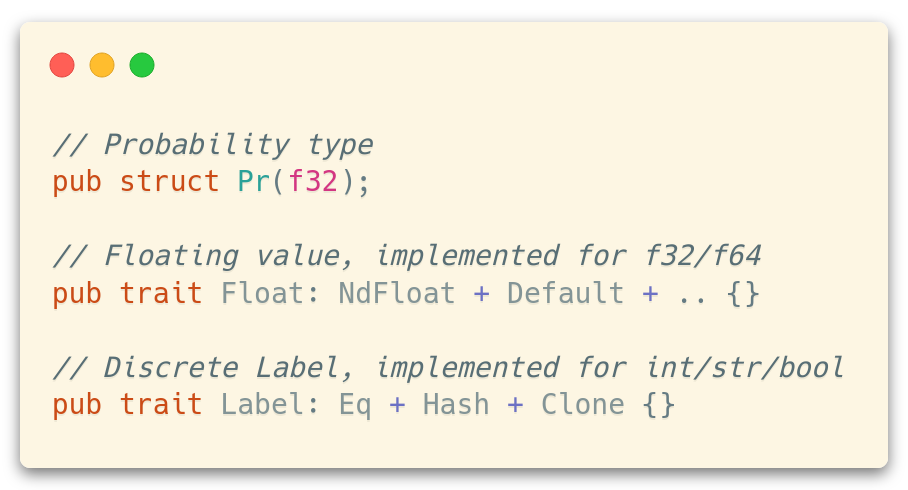
\includegraphics[width=0.5\linewidth]{images/types.png}
            \end{figure}
        }
    \end{itemize}

\end{frame}

\begin{frame}{metrics}
    \frametitle{Metric - Classification}

    \begin{itemize}
        \item<2-> Use confusion matrix as entry point to various classification metrics
            \only<2>{
                \begin{figure}[ht]
                    \centering
                    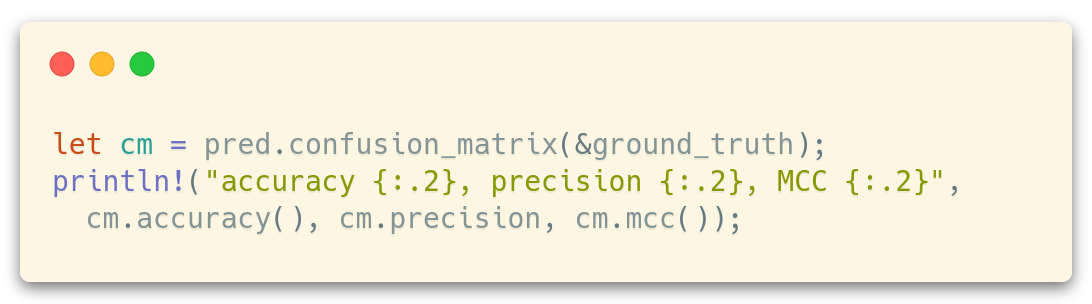
\includegraphics[width=0.8\linewidth]{images/metric_cm.png}
                \end{figure}
            }
        \item<3-> ROC curves for binary classifications
            \only<3>{
                \begin{figure}[ht]
                    \centering
                    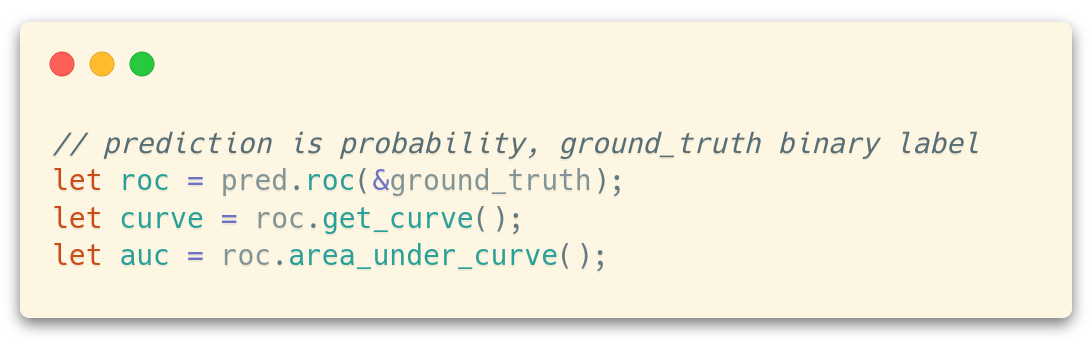
\includegraphics[width=0.8\linewidth]{images/metric_roc.png}
                \end{figure}
            }

    \end{itemize}

\end{frame}

\begin{frame}{example}
    \frametitle{Dataset - Examples}

    \begin{itemize}
        \item<1-> K-Folding
            \only<1>{
                \begin{figure}[ht]
                    \centering
                    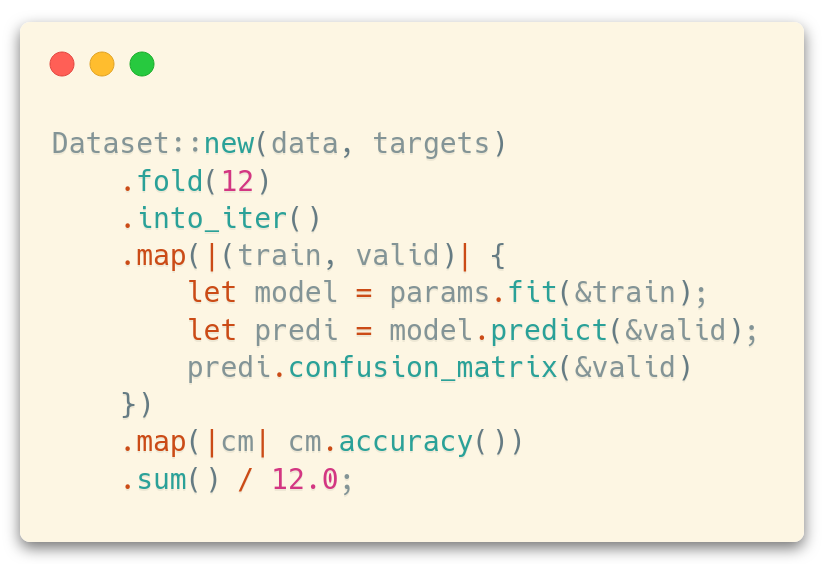
\includegraphics[width=0.8\linewidth]{images/kfolding.png}
                \end{figure}
            }
        \item<2-> One-vs-All
            \only<2>{
                \begin{figure}[ht]
                    \centering
                    \includegraphics[width=0.8\linewidth]{images/one_vs_all.png}
                \end{figure}
            }
    \end{itemize}
\end{frame}

\section{Case Studies}

\begin{frame}{kmeans}
    \frametitle{K-Means}

    \begin{itemize}
        \item<1-> First available algorithm, implemented at RustFest 2019
        \item<2-> Simple Expectation-Maximization optimization with hard assignment
        \item<3-> Done in two days, performance already improved when compared to \textit{Scikit-learn}
            \vspace{1em} \only<3>{
               \begin{table}[ht]
                   \centering
                    \begin{tabular}{ c | c }
                     Library & Training time \\
                     \hline \hline
                     Linfa & \SI{476.2}{ms} \\
                     Scikit-learn & \SI{604.7}{ms}
                    \end{tabular}
                    \caption{Mean training time for model of \SI{1}{mio} data points}
               \end{table}
           }
    \end{itemize}
\end{frame}

\begin{frame}{diffusionmaps}
    \frametitle{Diffusion maps}

    \begin{itemize}
        \item<1-> Connectivity as transition probability matrix $\mathbf{M}$
            \begin{align}
                \mathcal{P}(X_{t+1}=j|X_t=i) = M_{ij}
            \end{align}
        \item<2-> Where are we after $t$ steps, starting from node $v_i$
            \begin{align}
                v_i \to \mathbf{e}_i^T\mathbf{M}^t = (M_{i1}^{(t)},\dots,M_{in}^{(t)})
            \end{align}
        \item<3-> Perform spectral decomposition of $\mathbf{M}$ and project onto axis along it diffuses
    \end{itemize}
\end{frame}

\begin{frame}{diffusionexamplecode}
    \frametitle{Diffusion maps - Example}

    \begin{figure}[ht]
        \centering
        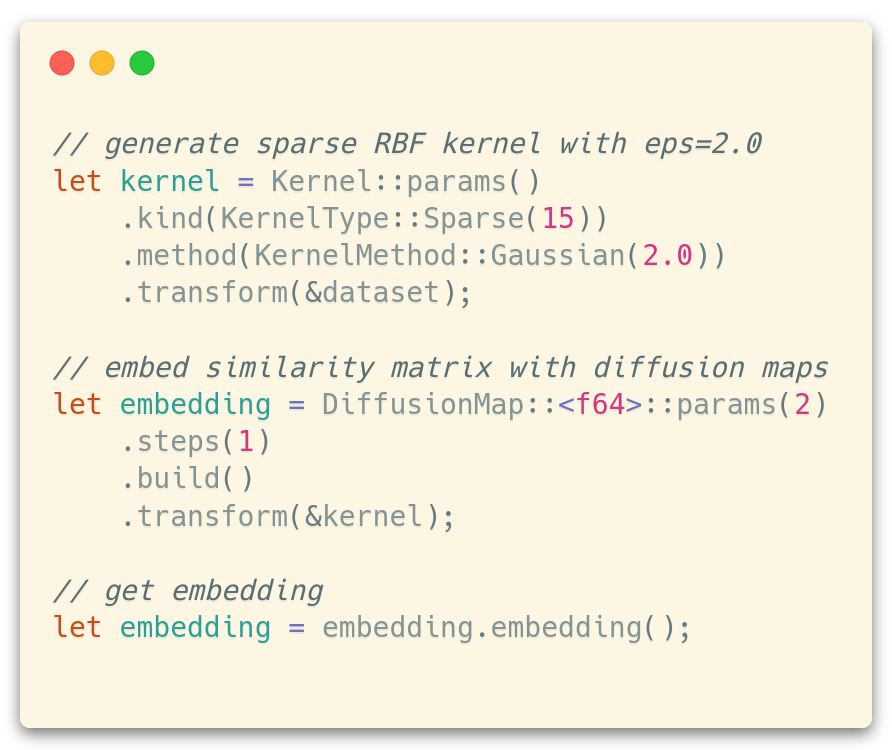
\includegraphics[width=0.5\linewidth]{images/diffusion_code.png}
        \caption{Kernel method and diffusion maps invocation in Linfa}%
    \end{figure}
\end{frame}

\begin{frame}{diffusionexample}
    \frametitle{Diffusion maps - Example}

    \begin{figure}[ht]
        \centering
        \subfloat[Original]{\resizebox{0.45\linewidth}{!}{\begin{tikzpicture}
\begin{axis}[%
scatter/classes={%
    a={mark=o,draw=black}},
    ticks=none,
]
\only<2->{
\addplot[scatter,only marks,%
    scatter src=explicit symbolic, blue]%
    table[x=x1, y=y1, col sep=comma] {images/scatter_original.dat};
}
\only<3->{
\addplot[scatter,only marks,%
    scatter src=explicit symbolic, green]%
    table[x=x2, y=y2, col sep=comma] {images/scatter_original.dat};
}

\only<4->{
\addplot[scatter,only marks,%
    scatter src=explicit symbolic, red]%
    table[x=x3, y=y3, col sep=comma] {images/scatter_original.dat};
}
\end{axis}
\end{tikzpicture}
}}
        \subfloat[Embedded]{\resizebox{0.45\linewidth}{!}{\begin{tikzpicture}
\begin{axis}[%
scatter/classes={%
    a={mark=o,draw=black}},
    ticks=none,
]
\only<2->{
\addplot[scatter,only marks,%
    scatter src=explicit symbolic, blue]%
    table[x=x1, y=y1, col sep=comma] {images/scatter_embedded.dat};
}
\only<3->{
\addplot[scatter,only marks,%
    scatter src=explicit symbolic, green]%
    table[x=x2, y=y2, col sep=comma] {images/scatter_embedded.dat};
}

\only<4->{
\addplot[scatter,only marks,%
    scatter src=explicit symbolic, red]%
    table[x=x3, y=y3, col sep=comma] {images/scatter_embedded.dat};
}
\end{axis}
\end{tikzpicture}
}}
        \caption{Nested rings and its transformation with diffusion maps.}%
    \end{figure}
\end{frame}

\begin{frame}{diffusionmaplob}
    \frametitle{Diffusion maps - LOBPCG}

    \begin{itemize}
        \item<2-> Locally Optimal Block Preconditioned Conjugate
            \only<2>{
            \begin{figure}[ht]
                \centering
                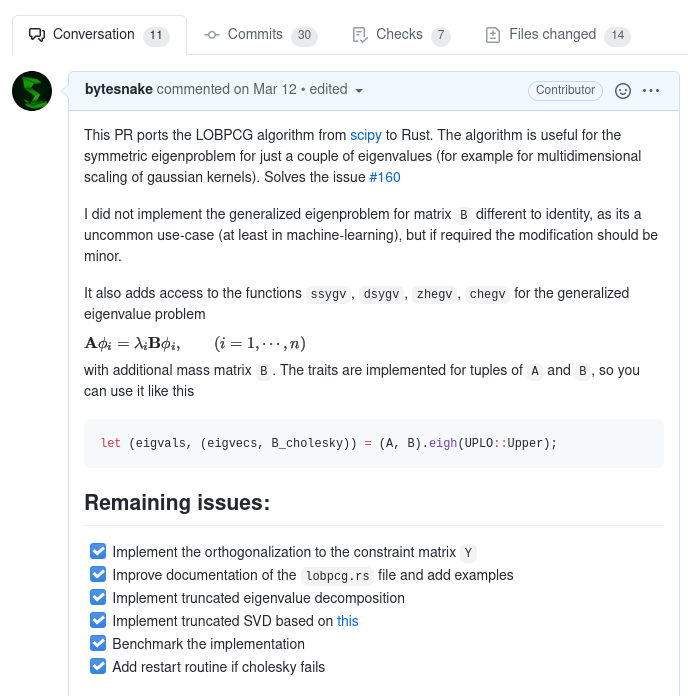
\includegraphics[width=0.6\linewidth]{images/lobpcg_github.png}
            \end{figure}
            }
            \begin{itemize}[label=-]
                \item<3-> useful for finding largest eigenvalues and corresponding eigenvectors
                \item<3-> factorization free, i.e. useful for sparse matrices
                \item<4-> matrix free, i.e. useful for covariance matrices
                \item<5-> linear convergence theoretically guaranteed
            \end{itemize}

            \only<6>{
            \begin{figure}[ht]
                \centering
                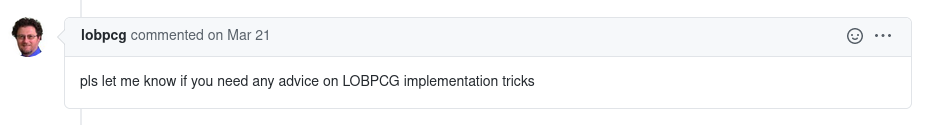
\includegraphics[width=0.9\linewidth]{images/lobpcg_author.png}
            \end{figure}
            }

    \end{itemize}
\end{frame}

\section{Summary}

\begin{frame}
    \frametitle{Available Algorithms}

    \begin{itemize}
        \item<1-> Clustering: K-Means, Gaussian Mixture, DBSCAN, \textit{Optics}
        \item<2-> Support Vector Machines: C/$\nu$/one-class classification and $\epsilon$/$\nu$ regression
        \item<3-> Reduction: PCA, diffusion maps and kernel methods
        \item<4-> Logistic regression
        \item<5-> Decision trees
        \item<6-> Hierarchical clustering
        \item<7-> Ordinary least squares, generalize linear models, \textit{elastic net}
        \item<8-> Fast Independent Component Analysis
        \item<9-> \textit{Gaussian Naive Bayes}
        \item<10-> \textit{Ensemble algorithms}, \textit{Random Forest}
    \end{itemize}
\end{frame}

\begin{frame}
    \frametitle{Next Steps}

    \begin{itemize}
        \item<2-> Good progress in Roadmap
        \only<2>{
            \begin{figure}[ht]
                \centering
                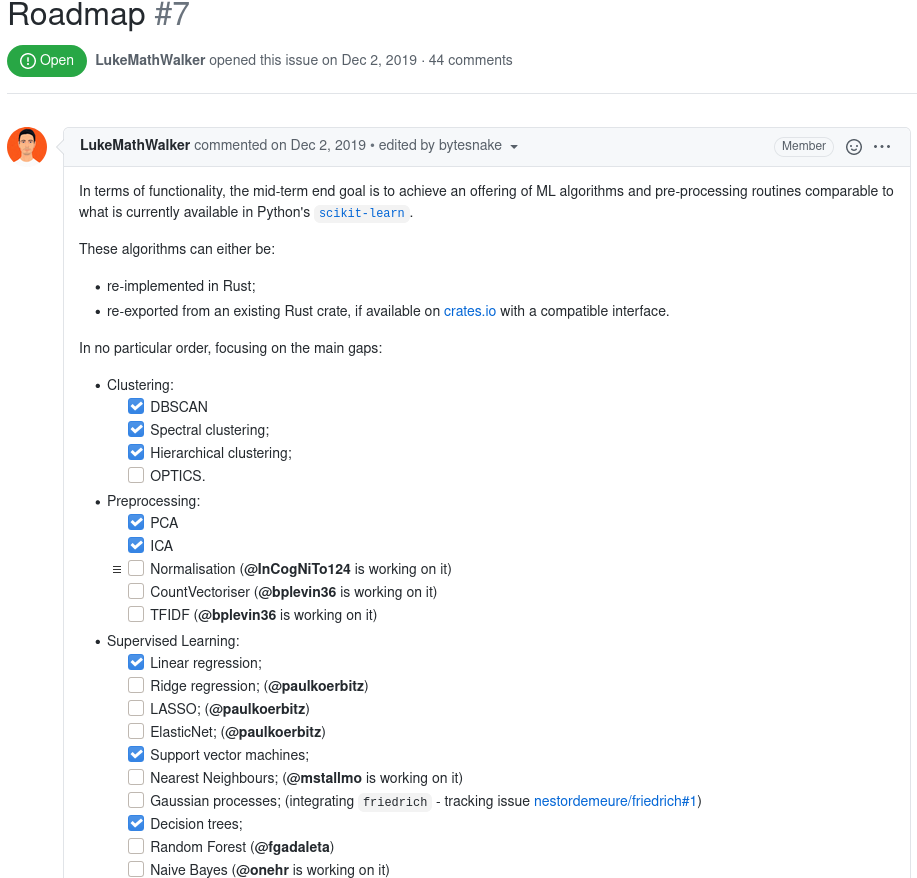
\includegraphics[width=0.8\linewidth]{images/roadmap.png}
            \end{figure}
        }
        \item<3-> But: Most algorithms only implement "the basics"
	\item<4-> Good testing is hard and still needs improvement
        \item<4-> Interfaces are currently being unified and polished
        \item<5-> We also need better documentation
        \item<6-> And most important of all: do some real-world experiments
    \end{itemize}

\end{frame}

\begin{frame}
	\centering \Large

	\emph{Thank you For Your Attention} 

    \vspace{5em}

    \only<2>{
        \emph{And To All Contributors}
        \vspace{1em}

        
\includegraphics[width=1.0\linewidth]{images/contributors.png}
    }
\end{frame}

\begin{frame}
    \frametitle{What is about AD and GPU?}

    \begin{itemize}
        \item<2-> Enzyme: Automatically generate differentiated functions in LLVM
            \only<2>{
                \begin{figure}[ht]
                    \centering
                    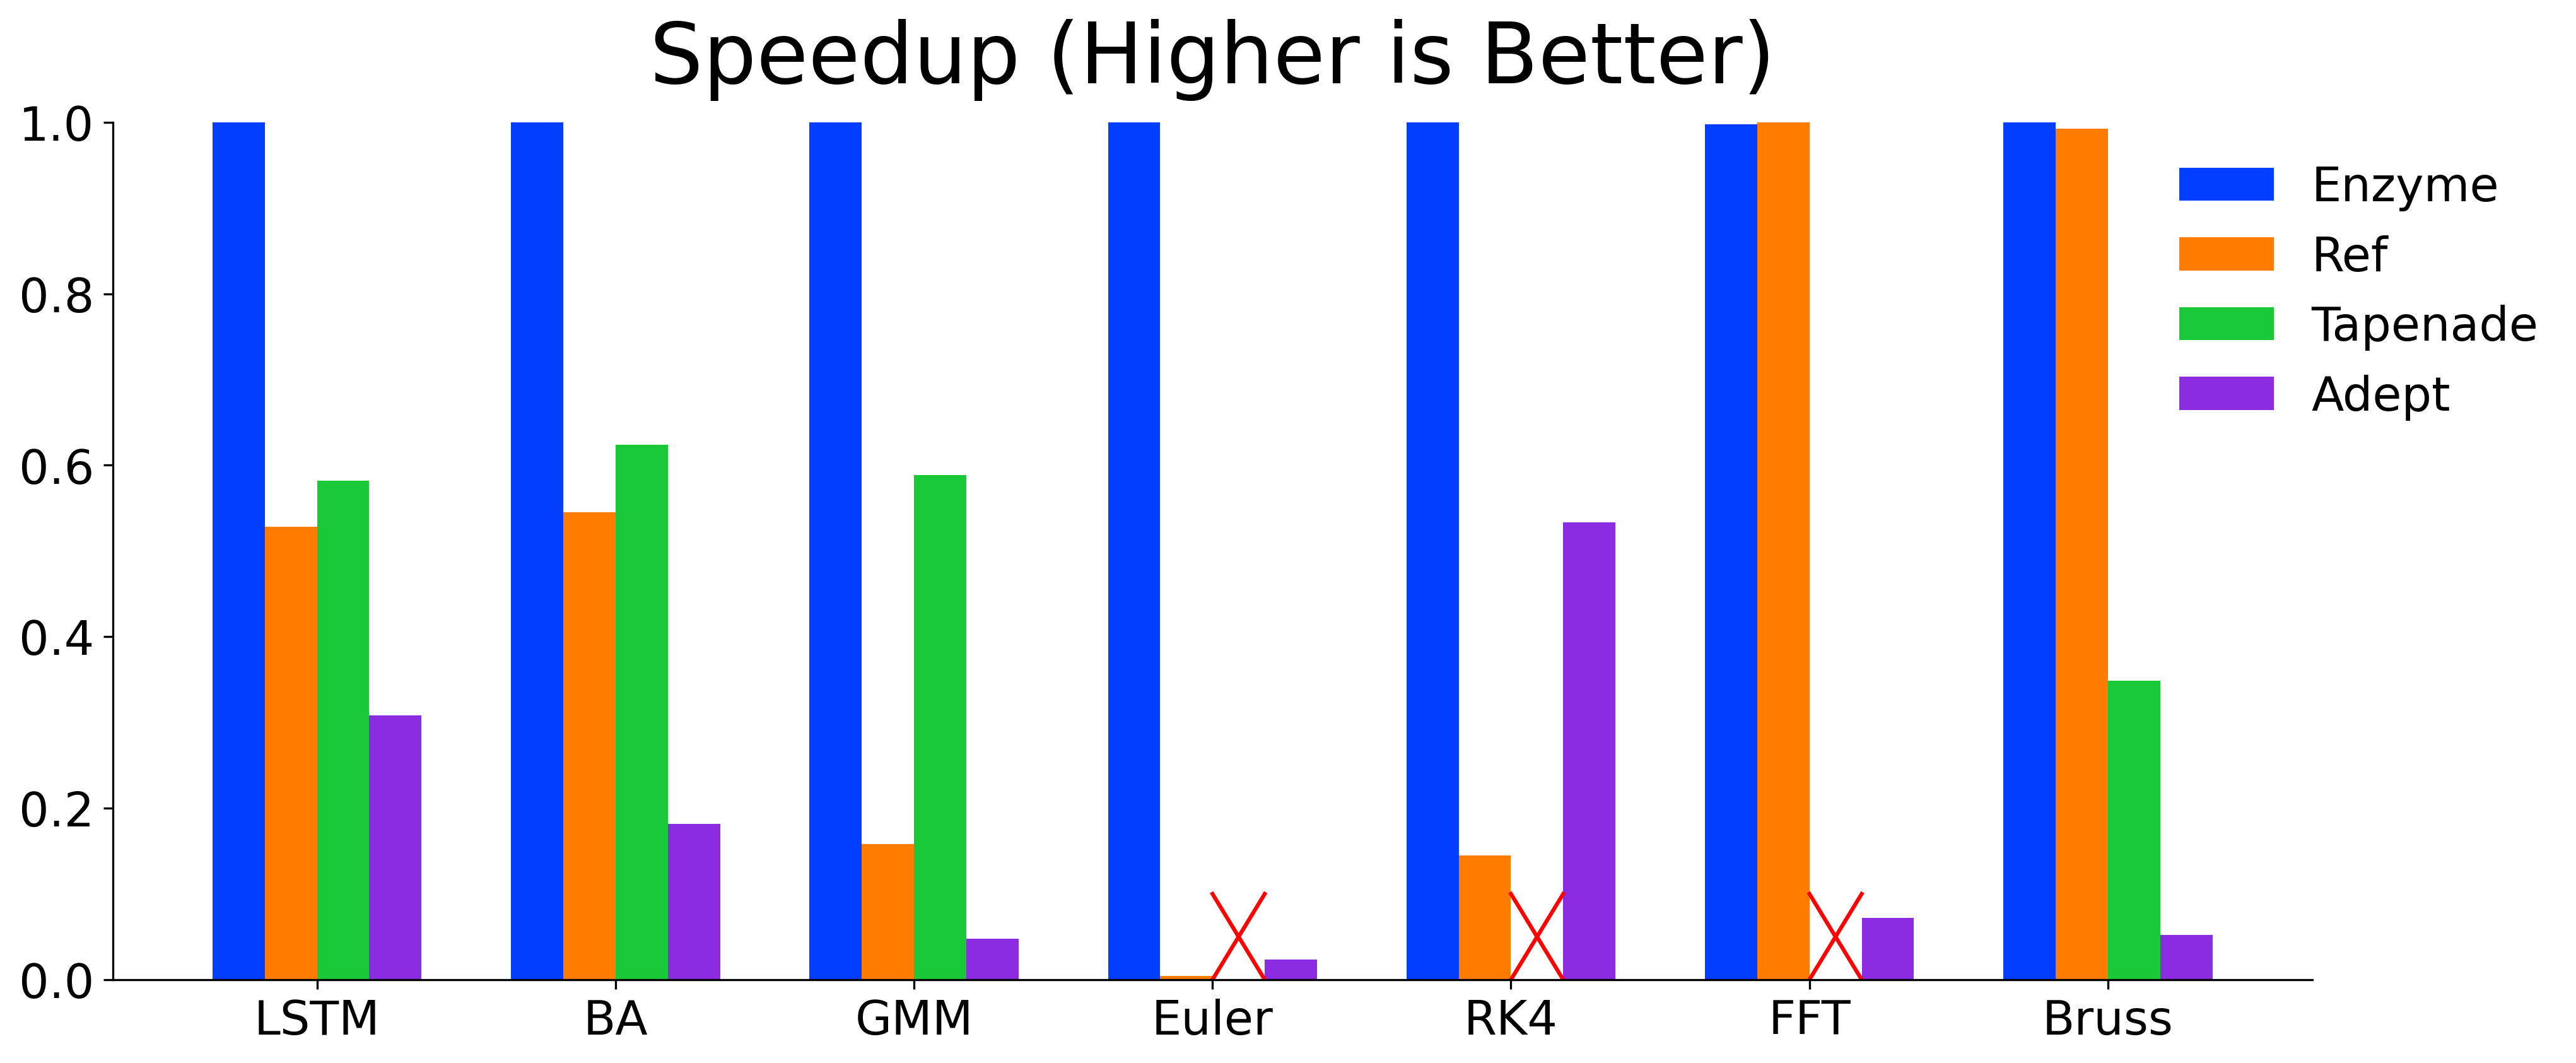
\includegraphics[width=0.8\linewidth]{images/enzyme.png}
                \end{figure}
            }
        \item<3-> Highly parallel execution on GPUs
    \end{itemize}
\end{frame}

%\begin{frame}[allowframebreaks]
%
%	\frametitle{References}
%
%	\bibliographystyle{amsalpha}
%
%	\bibliography{references.bib}
%
%\end{frame}
\end{document}
